\authoredSection{michael}{App-Idee}

\subsection{Problematik}
	Mit Rücksicht auf oben genannte Aspekte haben wir uns in der Ideenfindungsphase auf Lokalität als entscheidendes Schlagwort konzentriert. Apps wie etwa Yelp\footnote{\url{http://www.yelp.de/}, Abruf am 23.02.2014 um 16:15 Uhr, siehe auch Abbildung \ref{fig:Yelp}}, welche Bezug auf lokale Unternehmen nehmen und Benutzern die Möglichkeit geben, sich darüber auszutauschen, sind beispielhaft für eine erfolgreiche Umsetzung dieses Konzepts.
	
	Für das Bankgeschäft ergab sich jedoch das Problem, dass die eigenen finanziellen Verhältnisse in den innersten persönlichen Lebensbereich fallen und in der Regel darüber zumindest weniger Austausch stattfindet als über Restaurants, Nachtclubs oder Freizeitaktivitäten. So erschien es uns nachvollziehbar, dass die App eine Interaktion zwischen einem Kunden und einer Filiale begünstigen sollte, nicht aber den Austausch zwischen mehreren Kunden – der dann ohnehin wieder kaum eine Filiale benötigen würde.

\begin{figure}[h]
	\centering
	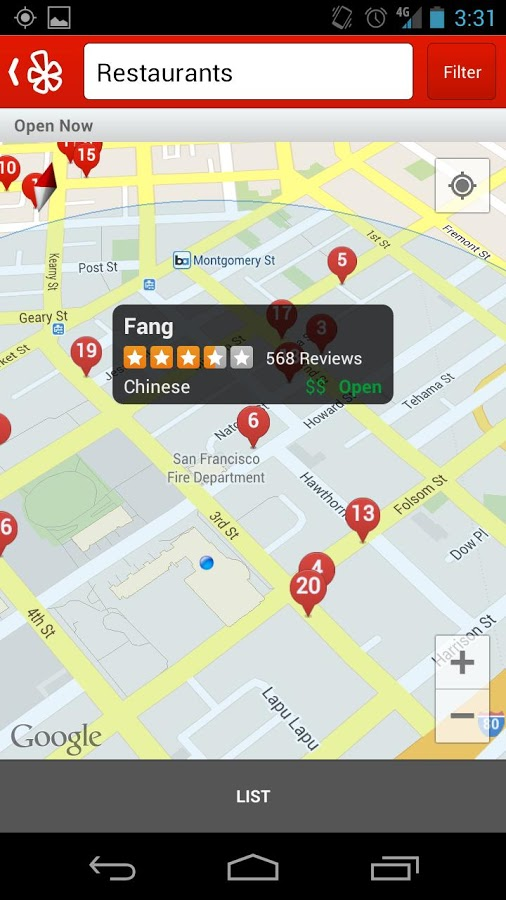
\includegraphics[scale=0.2]{Pictures/Yelp}
	\caption{Screenshot der Yelp-App \label{fig:Yelp}}
\end{figure}

	Erste Überlegungen zielten in Richtung interaktiver Beratungsdienstleistungen, welche jederzeit über Videotelefonie Kontakt zum individuell vertrauten Berater einer bestimmten Filiale herstellen sollten. In den wöchentlichen Diskussionen im Projektplenum wurden uns aber Mängel dieses Konzepts aufgezeigt; der individuelle Berater ist kein Alleinstellungsmerkmal der Filialbank mehr, eine virtuelle Filiale ist ohne weiteres denkbar.

	Allerdings, und hier haben wir die Chance unserer Anwendung gesehen, bedeutet die technische Möglichkeit eines Vertriebsweges nicht gleich, dass dieser auch angenommen wird. Eine von uns im Sinne einer Markterkundung durchgeführte Umfrage ergab ein gewisses Misstrauen gegenüber der Idee, Finanztransaktionen per App durchzuführen oder überhaupt eine Bank-App zu benutzen.
	
	Gründe hierfür könnten vielfältig sein; beispielsweise könnten die befragten Studenten am Informatikcampus eine besondere Sensibilität bezüglich Aspekten des Datenschutzes und der Transaktionssicherheit haben. Eine von der Unternehmensberatung „Bain and Company“ durchgeführte Studie zur Frage, wie digitalisierte Vertriebswege das Privatkundengeschäft der Banken zukünftig prägen könnten, ergab jedoch einen ähnlichen Tenor\footnote{\url{http://www.bain.de/Images/Retail\_Banking\_II\_Digitalisierung\_ES.pdf}, Abruf am 23.02.2014 um 16:30 Uhr.}.

	Insbesondere ergab die Studie, dass für Geldanlagen dem persönlichen Gespräch der Vorzug vor digitaler Beratung gegeben würde. Inwiefern eine solche Untersuchung aussagekräftig für eine Banking-App der Zukunft ist, sei dahingestellt. Schließlich wäre es auch möglich, dass hier einfach noch keine Gewöhnung stattgefunden hat und die Studie nur einen Übergangseffekt reflektiert, der für eine langfristig strategische Ausrichtung irrelevant wäre. 
 
	Bemerkenswert ist aber vielleicht auch, dass der Mensch in Finanzfragen nicht immer von Vernunft geleitet ist, sondern zunehmend auch nicht-funktionale Anforderungen in den Vordergrund stellt, wie etwa das Bedürfnis nach nachhaltigen Investitionen. Dies mag auch für die Art gelten, wie Finanzberatung vermittelt wird. Somit könnte es trotz aller technischen Möglichkeiten auch langfristig noch einen Markt für persönliche Beratung von Angesicht zu Angesicht geben.
 
\subsection{Vision}
	Schließlich entstand die Vision einer Anwendung, die nicht versucht, aus einer Filialbank eine Direktbank mit Filialen als Zusatzangebot zu machen, sondern die bestehenden Produkte des Filialgeschäfts dem Kunden näher bringt und ihm Grund gibt, in eine Filiale zu gehen. Dabei muss mit Blick auf die Stakeholder für Kunde und Bank ein Mehrwert geschaffen werden, der es für den Kunden rechtfertigt, eventuell höhere Gebühren als bei einer Direktbank zu bezahlen.

	Als Kernprodukte und Kompetenzen haben wir das klassische Sparbuch, die Anlageberatung sowie die Finanzierung ausgemacht. Das Sparbuch bietet scheinbar keine Funktionalität, die einen konkreten Vorteil gegenüber beispielsweise dem Tagesgeldkonto einer Direktbank hätte. Wie aber einführend erläutert, ist dies nicht ausschlaggebend. Denn ungeachtet seiner Nachteile ist das Sparbuch populär; vielleicht auch, weil in den Verwerfungen der europäischen Finanzkrise hier besondere Sicherheit vermutet wird. Tatsächlich ist aber ein Tagesgeldkonto bei einer Direktbank ebenso über die Einlagensicherung geschützt wie ein Sparbuch\footnote{Vgl. Einlagensicherungs- und Anlegerentschädigungsgesetz.}.

	Diesem Sicherheitsbedürfnis der Kunden wollten wir dabei konsequent nicht nur in der kryptographischen Theorie, sondern auch mit Rücksicht auf die vom Kunden wahrgenommene Sicherheit gerecht werden – etwa durch in der App prominente visuelle Elemente, die mit Sicherheit assoziiert werden.

	Filialbanken bieten heute sicher deutlich mehr an, als eben beschrieben. So kann man über ein bestimmtes Konto der Hamburger Sparkasse vergünstigte Reisen im eigenen Reise-Shop erwerben\footnote{Vgl. \url{https://www.haspajoker.de/index/Service/Reise-Service.html}, Abruf am 23.02.2014 um 16:45 Uhr.}; allerdings kann diese Expansion in andere Geschäftsfelder von der Fahrradversicherung bis zum Telefon-Rechtsschutz als Ausdruck wachsender Verzweiflung am schwindenden Kerngeschäft interpretiert werden. Diese als Webservice umgesetzten Zusatzangebote bilden aber wiederum keine Alleinstellungsmerkmale und sind daher von uns nicht integriert worden.

	In den nächsten Abschnitten wird nun erläutert werden, welche Funktionen wir uns in Konsequenz überlegt haben und mit welchen Use-Cases diese korrespondieren.

\subsection{Name}
    Der Name der App, „\textbf{K}i\textbf{B}a“, steht – in Anlehnung an eine bekannte Direktbank – ,für eine kundeninteressierte Bank, die mit der Anwendung mehr über ihre Kunden erfahren möchte und mit ihnen in Austausch treten will, um spezifischere Angebote und Beratungen anbieten zu können.
    
\subsection{Plattform}
    Bei der Erstellung eines konkreten Konzepts der Funktionalität haben wir zunächst die Anwendungsfälle besprochen, um die Frage nach der Plattform zu klären. Zweifelsohne gibt es Features, die in einem mobilen Anwendungsfall wahrscheinlicher sind, etwa das Auffinden einer Filiale oder eines Geldautomaten. Eine solche Funktionalität wäre aber nicht filialbankspezifisch. Überhaupt erschien es uns, als wäre der typische Anwendungsfall eher stationär, auf dem Sofa, im Büro, jedenfalls aber in Ruhe. Ein überzeugendes Argument für eine iPad-App ist auch, dass Kunde und Berater in der Filiale zusammen mit der App interagieren und Dinge visualisieren können.     
    
    Somit überwogen in der Gruppe ganz eindeutig die Argumente für eine iPad-Anwendung. Zudem war es Aufgabe, eine Vision für die Banking-App der Zukunft zu entwickeln. Der Trend geht unserer Meinung nach zum ubiquitären WLAN; so gibt es beispielsweise Bestrebungen, öffentliche Netzwerke in der Innenstadt einzurichten. Insofern darf davon ausgegangen werden, dass die mobile Konnektivität zukünftig auch beim iPad unproblematisch ist und somit webbasierte Funktionalität auch unterwegs gegeben ist.
    
\subsection{Funktionen}
\subsubsection{Finder}
	Ein intuitiv klarer Anwendungsfall ist der Wunsch eines Nutzers, die nächstliegende Filiale aus der App heraus auf einer Karte zu finden und dorthin navigieren zu können. Um diese Funktionalität noch gegenüber einem bekannten Kartendienst abzuheben, soll schon an dieser Stelle zusätzliche Interaktion mit einer Filiale möglich sein. Über eine Sortenanfrage können Devisen bestellt und aus der Filialseite, welche aus der Karte geöffnet wird, kann ein Termin vereinbart werden.

\subsubsection{Authentifizierung}
	Der Authentifzierungsmechanismus trennt die Funktionen in sicherheitsrelevante und unkritische. Ohne Authentifizierung steht dem Benutzer nur passive Funktionalität zur Verfügung, also etwa der Filialfinder oder die Umsatzanzeige. Um vom vollen Funktionsumfang der App profitieren zu können, muss der Benutzer in eine KiBa-Filiale gehen und von einem Berater einen Sicherheitscode eingeben lassen. Dieser garantiert dann in Kombination mit der App-ID der Anwendung eine eindeutige Zuordnung eines Benutzers an sein Gerät. Ähnlich einer Kreditkarte soll dann bei Verlust des Geräts auch die App selbst jederzeit gesperrt werden können. Insbesondere dient die Aktivierung aber auch dazu, den Kunden in einem Beratungsgespräch besser kennenzulernen und in einer Datenbank einen persönlichen Ansprechpartner festzuhalten.
	
\subsubsection{Self-Service}
	Im Zuge der Plenumsdiskussionen und anschließenden internen Debatten haben wir den zeitlichen Aspekt als zentrale Komponente identifiziert. Lokalität bedeutet, Dinge direkt zur Verfügung gestellt bekommen zu können. Viele Bescheinigungen und Unterlagen im täglichen Leben werden auch heute noch konkret ausgedruckt benötigt. Der typische Ablauf einer Direktbank sieht so aus, eine Anfrage – etwa nach Wertpapierzweitschriften oder Bonität – per Kontaktformular abzuschicken und dann einige Tage auf die entsprechenden Ausdrucke zu warten. Unsere Idee besteht in einer Self-Service-Station innerhalb der Bank, die das Konzept bestehender Automaten erweitert.
	
\begin{figure}
	\centering
	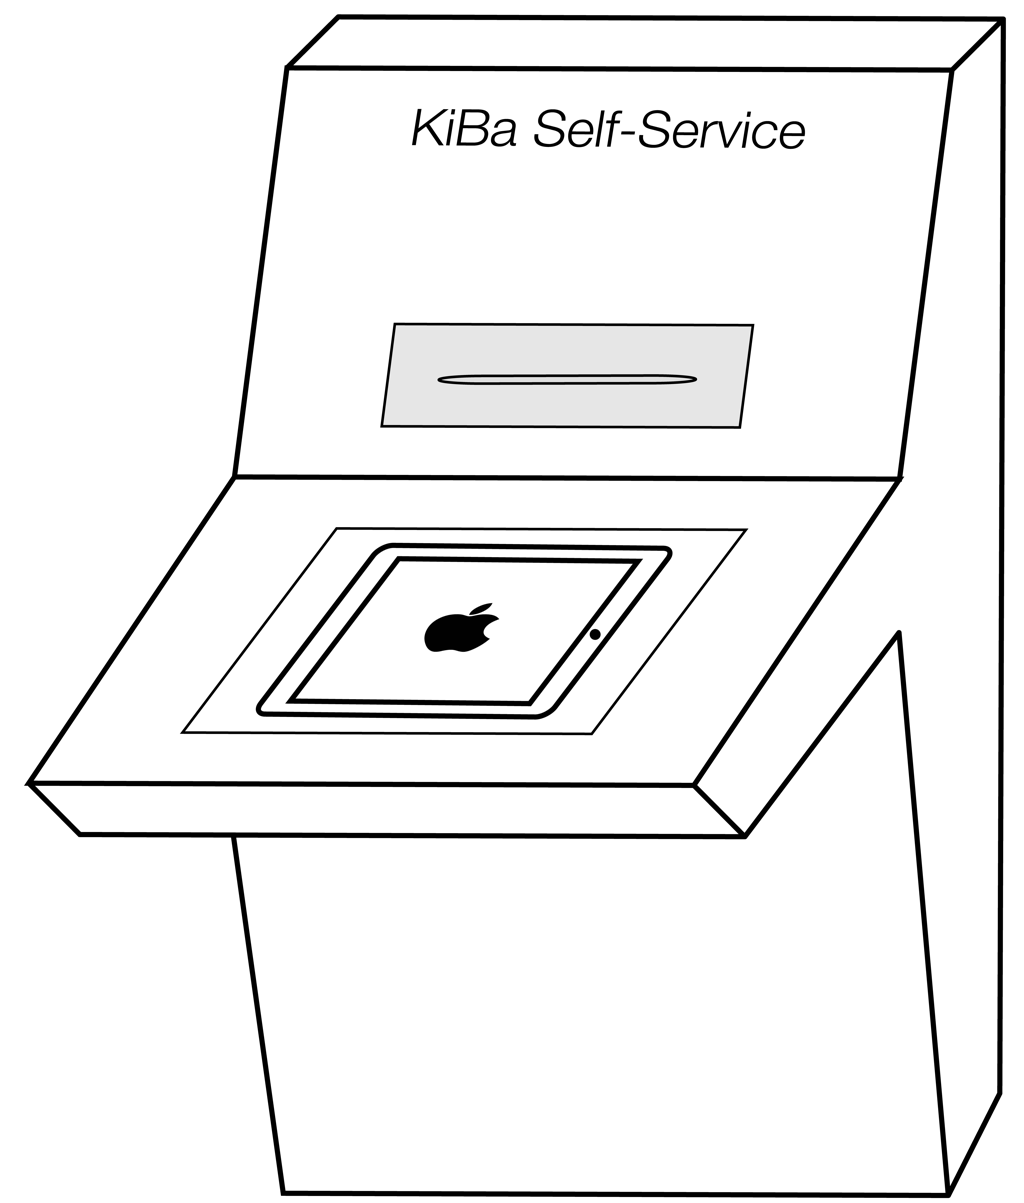
\includegraphics[scale=0.2]{Pictures/SelfService}
	\caption{Piktogramm unserer Self-Service-Station\label{fig:SelfService}}
\end{figure}
	
	Ein Kunde kann sein iPad auf eine Ablage legen und sich mit der Station verbinden, welche eine Art Multifunktionsdrucker beinhaltet, vergleiche Abbildung \ref{fig:SelfService}. Über die App können dann verschiedenste Bescheinigungen ausgedruckt und Konten eröffnet werden. Das entscheidende dabei ist, dass der Kunde durch die Authentifizierung in einer Filiale seinem Gerät zugeordnet wurde. Somit können an derartigen Stationen auch Interaktionen vorgenommen werden, die normalerweise die Identifikation per Lichtbildausweis am Schalter erfordern würden. Somit entsteht hier Mehrwert für alle Stakeholder: Kunden müssen weniger anstehen für standardisierte Abläufe, die Bank spart unter Umständen Personalkosten und kann Mitarbeiter für das Wesentliche, die Beratung, einsetzen.

   Umbuchungen am Sparbuch können üblicherweise nur in einer Filiale vorgenommen werden, überwiesen werden kann nur auf das Sparkonto. Die Greifbarkeit des Sparbuches vermittelt konservativen, besorgten Sparern ein Gefühl von Sicherheit. Gleichzeitig kann es aber durch diese funktionale Einschränkung auch zu unerwünschten Situationen kommen: ist etwa durch eine Fehlkalkulation an einem Samstagabend kein Geld mehr auf dem Girokonto, muss bis zur Öffnung einer Filiale am Montag gewartet werden, um Guthaben umbuchen zu können. Um dem vorzubeugen, soll über die Self-Service-Station auch Geld umgebucht werden können. Da die Station im Vorraum der Filiale steht, ist sie immer zugänglich.   
    
\subsubsection{Individueller Finanzierungsrechner}
	Wie oben erläutert, besteht eine wesentliche Dienstleistung von Filialbanken in der Finanzierung, etwa für Eigenheime. Im Zentrum unserer Überlegungen stand dann auch die Frage, wie eine App dabei helfen kann, diese Dienstleistung für den Endkunden zu verbessern.
	
	Im Ergebnis möchten wir einen individualisierten Kreditrechner anbieten, der den App-Benutzer in die Lage versetzt, mittels individuell berechneter Profildaten für sich selbst Finanzierungsrechnungen durchzuführen. Die Idee dahinter ist, dass ein Kunde zunächst für sich selbst einige Finanzierungsvarianten durchspielen kann. Hat er sich für eine Variante entschieden, kann ein Termin mit dem persönlichen Berater vereinbart werden. Im Filialgespräch kann der Berater dann noch individuelle Ratschläge bezüglich Laufzeit und Umfang einer Finanzierung geben. Wichtig dabei ist, dass die angebotenen Finanzierungsdaten  mit Rücksicht auf die der Bank zur Verfügung stehenden Informationen so konservativ gewählt sind, dass sie in jedem Falle von der Bank eingehalten werden können.
 
\subsubsection{Weitere Funktionen}
    Als Startbildschirm nach dem Login ist für die App ein Dashboard vorgesehen, das einen graphischen Überblick über Vermögensverlauf und Transaktionen bereitstellt. Hilfreich war hier die Überlegung, dass die meisten Benutzer ihren Kontostand grob kennen und weniger an einer Zahl als vielmehr an den Entwicklungen interessiert sind. Zudem gibt es einen Nachrichtenbereich, in dem die Antworten auf beispielsweise Terminanfragen abgelegt werden. Einfache Überweisungen können ebenfalls getätigt werden, schlicht, weil dies unserer Ansicht nach von einer Bankanwendung erwartet wird.
    